% Experiments. Numbers: refs/internal/html-report/data.json (v12, asr, babble,
% qwen3_hotwords) and supp.json (bench, hwv3), identical to the published HTML §6.
% Headline numbers re-derived from the AmphionEval records (fact-check block).
% Organization follows the headline-table + condition-breakdown layout of the
% 1.0 report §5 and Seed-ASR, per AGENTS.md rule 6.

\section{Experiments}
\label{sec:experiments}

\subsection{Setup}
\label{subsec:exp_setup}

\paragraph{Test sets.}
\Cref{tab:testsets} lists the test sets.
TS-ASR is evaluated on \tsbench (\Cref{sec:benchmark}); the other capabilities are evaluated on public test sets and in-house test sets.

\paragraph{Normalization and metrics.}
Mandarin normalization and the three TS-ASR metrics are defined in \Cref{subsec:bench_metrics}.
English is scored by word after the Whisper English normalizer~\cite{radford2023robust}.

\paragraph{Inference.}
AmphionASR~2.0 is served with vLLM~\cite{kwon2023vllm}, with greedy decoding, at most 512 generated tokens and the first 5\,s of each enrollment.
Every test set is evaluated on all of its items.

\paragraph{Baselines.}
For TS-ASR we compare with Xiaomi-CocktailASR-1~\cite{zhang2026xiaomi} in both its standard and its chain-of-thought (CoT) mode.
Of the related systems in \Cref{tab:design}, it is the only external one that transcribes a single enrolled speaker in Mandarin and outputs nothing when that speaker is absent.
MT-LLM is trained on English and German, SpeakerLM transcribes every speaker of a conversation, and DiCoW takes diarization output instead of an enrollment.
The CocktailASR-1 report does not link released weights, so we use those published on Hugging Face as \texttt{Ease3/Xiaomi-CocktailASR-1}, with the transformers inference code that comes with them (bf16, greedy decoding).
CocktailASR-1 runs on the same audio, the same first 5\,s of enrollment and the same scoring as AmphionASR~2.0.
That report samples the reference speech at random lengths of 1--4\,s.
On an earlier version of our test set, a fixed 3\,s crop and such a random crop gave group CERs that differed by at most about 7 points and essentially the same target-absent false-alarm rates.
For plain ASR we compare with Qwen3-ASR-1.7B~\cite{shi2026qwen3asr}, MiMo-V2.5-ASR, Ming-3.0-asr-tiny, VibeVoice-ASR-7B and Dolphin-CN-Dialect; all baseline numbers are measured by us on the same data with the same scoring.
% TODO: add citations for MiMo-V2.5-ASR, Ming-3.0-asr-tiny, VibeVoice-ASR-7B and
% Dolphin-CN-Dialect (official model cards); none is in refs INDEX yet.

\begin{table}[t]
  \caption{Test sets used in this report.}
  \label{tab:testsets}
  \centering
  \small
  \begin{tabularx}{\linewidth}{@{}l>{\raggedright\arraybackslash}X>{\raggedright\arraybackslash}p{3.0cm}@{}}
    \toprule
    Capability & Test set & Metrics \\
    \midrule
    TS-ASR & \tsbench (\Cref{sec:benchmark}): 24{,}101 samples in 248 subsets; synthetic degraded enrollment, entry and exit, short segments, noise and far field; real AliMeeting, AISHELL-4 and MagicData-RAMC test windows and web conversations & CER, empty-output rate, false-alarm rate \\
    Babble robustness & In-house, 16 splits $\times$ 200 samples & false-alarm rate, CER, WER \\
    Hotword ASR & AISHELL-1 and Common Voice English hotword subsets (correct word plus 10 distractors); in-house retrieved-candidate test (264{,}681 requests) & CER, WER, hotword recall, false-alarm rate \\
    Plain ASR & AISHELL-1~\cite{bu2017aishell1}, AISHELL-2~\cite{du2018aishell2}, AISHELL-3~\cite{shi2021aishell3}, MagicData, THCHS-30~\cite{wang2015thchs30}, KeSpeech~\cite{tang2021kespeech}, Common Voice~\cite{ardila2020common}, WenetSpeech~\cite{zhang2022wenetspeech}, LibriSpeech~\cite{panayotov2015librispeech}, MLS~\cite{pratap2020mls}, GigaSpeech~\cite{chen2021gigaspeech}, TALCS~\cite{li2022talcs}, WenetSpeech-Chuan, CHiME-4~\cite{vincent2017analysis} & CER, WER \\
    \bottomrule
  \end{tabularx}
\end{table}

\subsection{Target-speaker recognition}
\label{subsec:exp_tsasr}

\Cref{tab:ts_overall} gives the overall results on \tsbench.
With the target present, AmphionASR~2.0 reaches 13.1\% CER, about two fifths of the 33.4\% of CocktailASR-1, at a similar empty-output rate (2.9\% and 2.7\%).
The largest gap is with the target absent: the false-alarm rates of AmphionASR~2.0 are 3.8\% on synthetic scenes and 2.6\% on real conversations, against 64.5\% and 96.1\% for CocktailASR-1.
With chain of thought enabled, CocktailASR-1 reaches 39.6\% CER on target-present samples and a 61.9\% false-alarm rate on target-absent samples.
These numbers compare whole systems: no controlled experiment in this report separates the contribution of the training data from that of the architecture or the model size.
The same team also built \tsbench and the training data of AmphionASR~2.0.
Training scene types such as turn-taking, hand-overs, short sentences and similar voices also appear in the benchmark, and the real part measures in-domain behavior for AmphionASR~2.0 because the training splits of its corpora are used in training (\Cref{sec:limitations}).

\begin{table}[t]
  \caption{Overall TS-ASR results on \tsbench (\%, lower is better). Bold marks the best value in each row.}
  \label{tab:ts_overall}
  \centering
  \small
  \begin{tabular}{@{}lccc@{}}
    \toprule
    Metric & AmphionASR 2.0 & CocktailASR-1 & CocktailASR-1 $\cdot$ CoT \\
    \midrule
    Target present $\cdot$ CER & \best{13.1} & 33.4 & 39.6 \\
    Target present $\cdot$ empty output & 2.9 & \best{2.7} & 3.0 \\
    Target absent $\cdot$ false alarm (all) & \best{3.7} & 67.8 & 61.9 \\
    \quad synthetic scenes & \best{3.8} & 64.5 & 58.8 \\
    \quad real meetings, calls and web conversations & \best{2.6} & 96.1 & 87.7 \\
    \midrule
    Real conversations $\cdot$ target-present CER & \best{9.2} & 30.8 & 27.2 \\
    Target alone, one 2--6\,s sentence $\cdot$ CER & 5.5 & 4.1 & \best{3.6} \\
    Four others speaking, target absent $\cdot$ false alarm & \best{8.3} & 89.2 & 77.5 \\
    Babble only $\cdot$ false alarm & \best{3.3} & 29.2 & 75.0 \\
    \bottomrule
  \end{tabular}
  \par\smallskip
  {\footnotesize 24{,}101 samples in 248 subsets (12{,}950 target-present, 11{,}151 target-absent); the first 5\,s of each enrollment recording are used. CER is pooled over all target-present samples; the empty-output and false-alarm rates are counted per sample.\par}
\end{table}

\begin{figure}[t]
  \centering
  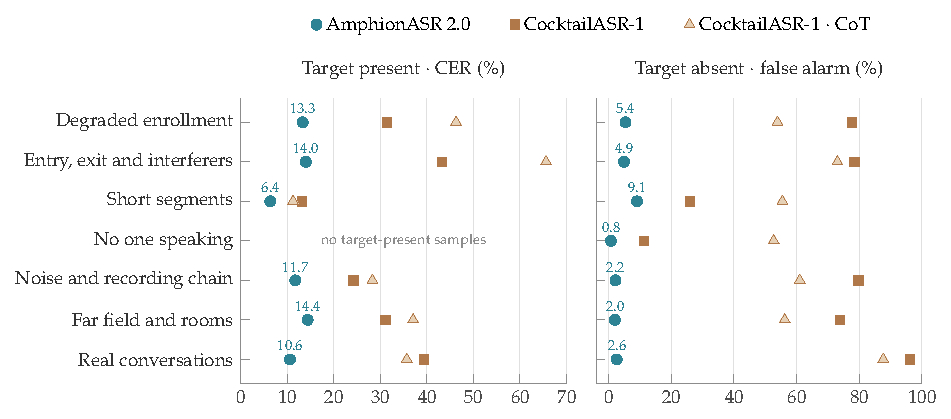
\includegraphics[width=\linewidth]{figures/section-results.pdf}
  \caption{Results pooled by section of \tsbench. Left: target-present CER; right: target-absent false-alarm rate. The ``no one speaking'' section has target-absent samples only. \Cref{app:scenarios} gives the results by scenario.}
  \label{fig:sections}
\end{figure}

By section (\Cref{fig:sections}), AmphionASR~2.0 has a lower target-present CER than CocktailASR-1 in every section, and a target-absent false-alarm rate more than an order of magnitude lower in every section except short segments.
The false alarms of CocktailASR-1 are concentrated in conditions where other people talk at length.
Its false-alarm rate is about 11\% when nobody speaks and 11.0\% on 1.2--6\,s segments with only others speaking, against 71.8--100\% in the target-absent groups of all other sections except short segments (\Cref{tab:scenarios}).
When the target alone says one short sentence, the two systems have similar CER (4.2\% and 4.8\%).

\subsection{How the evaluation conditions change the conclusion}
\label{subsec:exp_conditions}

\Cref{tab:conditions} regroups the subsets of \tsbench by whether common evaluations also cover them.
The first four rows are cases that common evaluations can measure: only the target speaking, nobody speaking, and the target mixed with one interferer.
With only the target speaking, all three systems stay at or below 7.5\% CER, and they are almost identical on real recordings; the CoT mode even has the lowest CER in the synthetic condition (3.8\%).
If an evaluation also includes target-absent samples in which nobody speaks, as the evaluation of AmphionASR~1.0 did, CocktailASR-1 has a false-alarm rate of 10.8\%, which looks acceptable.
The usual two-talker mixture does separate the target-present CERs (7.3\% and 21.3\%) but still misses the main difference.
With others talking and the target absent, CocktailASR-1 transcribes someone else on 85.8\% of synthetic and 96.1\% of real samples, against 3.5\% and 2.6\% for AmphionASR~2.0.
With the target present and 2--4 interferers, the CER of CocktailASR-1 rises to 65.7\%, against 18.9\% for AmphionASR~2.0.

\begin{table}[t]
  \caption{How the evaluation conditions change the conclusion (\%, lower is better). Bold marks the best value in each row.}
  \label{tab:conditions}
  \centering
  \small
  \begin{tabularx}{\linewidth}{@{}>{\raggedright\arraybackslash}Xrccc@{}}
    \toprule
    Condition & Samples & AmphionASR 2.0 & CocktailASR-1 & CoT \\
    \midrule
    \multicolumn{5}{@{}l}{\textit{Conditions that common evaluations also cover}} \\
    Only the target speaks $\cdot$ synthetic $\cdot$ CER & 540 & 4.6 & 5.5 & \best{3.8} \\
    Only the target speaks $\cdot$ real windows $\cdot$ CER & 194 & 7.5 & \best{7.3} & 7.5 \\
    Nobody speaks $\cdot$ false alarm & 720 & \best{0.1} & 10.8 & 58.1 \\
    Target + 1 interferer, target present $\cdot$ CER & 480 & \best{7.3} & 21.3 & 61.3 \\
    \midrule
    \multicolumn{5}{@{}l}{\textit{Conditions common in real use but not covered by common evaluations}} \\
    Target + 2--4 interferers, target present $\cdot$ CER & 1{,}080 & \best{18.9} & 65.7 & 86.5 \\
    Real windows with 3+ talkers, target present $\cdot$ CER & 126 & \best{18.1} & 64.7 & 40.3 \\
    Others speaking, target absent $\cdot$ synthetic $\cdot$ false alarm & 480 & \best{3.5} & 85.8 & 66.7 \\
    Others speaking, target absent $\cdot$ real recordings $\cdot$ false alarm & 1{,}191 & \best{2.6} & 96.1 & 87.7 \\
    A similar-sounding person speaking, target absent $\cdot$ false alarm & 540 & \best{18.0} & 73.9 & 89.3 \\
    \bottomrule
  \end{tabularx}
  \par\smallskip
  {\footnotesize Synthetic ``only the target speaks'': 3 subsets (a whole clip, one short phrase, one 2--6\,s sentence); ``target + 1 interferer'': 4 subsets (continuous speech, simultaneous start, interjection, about 1\,s of speech); ``target + 2--4 interferers'': 9 subsets; ``nobody speaks'': 6 subsets (noise, music, traffic, near silence, very short and long clips); synthetic ``others speaking'': 4 subsets (1, 2 and 4 interferers, long clips); ``similar-sounding person'': 3 subsets. Target-present rows on real windows use clean enrollments only; the real target-absent row covers all target-absent samples of the real-conversation section. CoT: CocktailASR-1 in chain-of-thought mode.\par}
\end{table}

\paragraph{Paired subsets locate weaknesses.}
Two groups of target-absent samples are paired: the mixture is identical item by item, and only the enrollment changes, to that of a random person or of someone who sounds like a speaker in the mixture.
With a random enrollment, false alarms from AmphionASR~2.0 are rare (0.0\% on 6--18\,s segments and 4.7\% on one short phrase); with a similar-sounding enrollment, the rates rise to 12.5\% and 22.7\%.
This is the main remaining weakness of AmphionASR~2.0 (\Cref{sec:limitations}), and an evaluation that enrolls only random people would not reveal it.

\paragraph{Synthetic conditions against real recordings.}
The same AliMeeting windows exist as near-field and far-field recordings, which lets us check the synthetic far-field conditions against real ones (\Cref{tab:nearfar}).
The two agree on enrollment--mixture mismatch: with a far-field enrollment and a near-field mixture, the empty-output rate of AmphionASR~2.0 rises from 2.5\% to 6.7\% on synthetic data and from 0.9\% to 5.2\% on real recordings.
The synthetic far-field mixture, however, is harsher than a real meeting room.
With a near-field enrollment, switching the mixture to far field raises CER from 8.6\% to 16.9\% on synthetic data but only from 4.5\% to 6.4\% on real recordings.
We therefore use the synthetic subsets to find which factors the model is sensitive to, and the real subsets to measure how large the effects are.

\begin{table}[t]
  \caption{Synthetic far-field conditions against real recordings (AmphionASR~2.0, target present, CER / empty output, \%).}
  \label{tab:nearfar}
  \centering
  \small
  \begin{tabular}{@{}lcc@{}}
    \toprule
    Enrollment $\cdot$ mixture & Synthetic & Real AliMeeting \\
    \midrule
    Near-field enrollment $\cdot$ near-field mixture (baseline) & 8.6 / 2.5 & 4.5 / 0.9 \\
    Near-field enrollment $\cdot$ far-field mixture & 16.9 / 1.7 & 6.4 / 1.7 \\
    Far-field enrollment $\cdot$ near-field mixture & 10.6 / 6.7 & 10.7 / 5.2 \\
    Far-field enrollment $\cdot$ far-field mixture & 20.6 / 3.3 & 6.8 / 0.9 \\
    \bottomrule
  \end{tabular}
  \par\smallskip
  {\footnotesize Synthetic: the same base scenes (target plus one or two interferers), far field from measured room responses, 120 samples per cell. Real: the same 115 AliMeeting test windows, clean enrollments only; near field is the speaker's headset microphone, the near-field mixture is the sum of all headsets (level-matched to the far-field mixture), and far field is the first array channel.\par}
\end{table}

\subsection{Real meetings, phone calls and web conversations}
\label{subsec:exp_real}

The windows in \Cref{tab:real} are taken directly from the test sets of public corpora.
The false-alarm rate per corpus is 1--5\% for AmphionASR~2.0 and 74--100\% for CocktailASR-1.
With the target present, CocktailASR-1 also has a higher CER, for example 38.2\% on AliMeeting against 6.8\% for AmphionASR~2.0.
When the enrollment clip contains another voice, the target-present CER of AmphionASR~2.0 is 6--11 points higher than with a clean enrollment, while its target-absent false-alarm rate does not rise.

\begin{table}[t]
  \caption{Real meetings, phone calls and web conversations (\%). Target-present rows give CER / empty output; target-absent rows give the false-alarm rate. Bold marks the best value in each row.}
  \label{tab:real}
  \centering
  \small
  \begin{tabularx}{\linewidth}{@{}>{\raggedright\arraybackslash}Xrccc@{}}
    \toprule
    Corpus and condition & Samples & AmphionASR 2.0 & CocktailASR-1 & CoT \\
    \midrule
    AliMeeting far-field meetings (present) & 115 & \best{6.8 / 0.9} & 38.2 / 0.0 & 36.9 / 0.0 \\
    AliMeeting far-field meetings (absent) & 100 & \best{1.0} & 100.0 & 97.0 \\
    AISHELL-4 far-field meetings (present) & 141 & \best{15.0 / 5.0} & 27.7 / 0.0 & 23.0 / 0.0 \\
    AISHELL-4 far-field meetings (absent) & 140 & \best{5.0} & 100.0 & 97.1 \\
    MagicData-RAMC phone calls (present) & 100 & \best{13.3 / 0.0} & 16.1 / 0.0 & 16.0 / 0.0 \\
    MagicData-RAMC phone calls (absent) & 100 & \best{5.0} & 96.0 & 83.0 \\
    Emilia web conversations, pseudo-labels (present) & 148 & \best{10.2 / 2.0} & 19.7 / 0.0 & 16.6 / 0.0 \\
    Emilia web conversations, pseudo-labels (absent) & 150 & \best{2.7} & 74.0 & 50.0 \\
    AliMeeting near/far-field pairs (present) & 460 & \best{7.1 / 2.2} & 36.3 / 0.0 & 31.5 / 0.2 \\
    AliMeeting near/far-field pairs (absent) & 400 & \best{2.0} & 99.8 & 90.5 \\
    \midrule
    Real meetings $\cdot$ enrollment contains another voice (present) & 62 & \best{15.6 / 1.6} & 60.8 / 0.0 & 64.1 / 0.0 \\
    Real meetings $\cdot$ enrollment contains another voice (absent) & 77 & \best{1.3} & 97.4 & 96.1 \\
    AliMeeting pairs $\cdot$ enrollment contains another voice (present) & 164 & \best{18.5 / 4.9} & 94.1 / 0.0 & 87.0 / 0.6 \\
    AliMeeting pairs $\cdot$ enrollment contains another voice (absent) & 224 & \best{2.2} & 100.0 & 96.9 \\
    \bottomrule
  \end{tabularx}
  \par\smallskip
  {\footnotesize Windows are cut directly from the human-annotated test sets of AliMeeting, AISHELL-4 and MagicData-RAMC and from Emilia web conversations, without mixing; Emilia references come from automatic diarization and recognition. ``Enrollment contains another voice'' means that another speaker talks for at least 0.3\,s within the first 5\,s of the enrollment clip.\par}
\end{table}

\subsection{Enrollment quality}
\label{subsec:exp_enrollment}

\Cref{tab:enrollment} changes only the enrollment on the same base scenes.
Another voice mixed into the enrollment has the largest effect, whereas leading silence, narrowband audio, a noise floor and reverberation change the results of AmphionASR~2.0 little.
With only 1\,s of speech in the enrollment, the target-absent false-alarm rate rises to 23.3\%.
During development we also swept the enrollment length: 3\,s and 5\,s both work, while 8\,s or more increases the empty-output rate with the target present; this observation has not been analyzed further.

\begin{table}[t]
  \caption{Effect of enrollment quality (\%). For each system: target-present CER, target-present empty-output rate and target-absent false-alarm rate.}
  \label{tab:enrollment}
  \centering
  \small
  \begin{tabular}{@{}lcccccc@{}}
    \toprule
    & \multicolumn{3}{c}{AmphionASR 2.0} & \multicolumn{3}{c}{CocktailASR-1} \\
    \cmidrule(lr){2-4}\cmidrule(l){5-7}
    Enrollment & CER & Empty & FA & CER & Empty & FA \\
    \midrule
    Clean enrollment & 11.9 & 2.7 & 0.7 & 20.9 & 0.7 & 74.0 \\
    Only 1\,s of speech (rest zero-padded) & 19.8 & 2.0 & 23.3 & 86.1 & 8.0 & 85.3 \\
    Leading silence & 11.4 & 0.7 & 2.0 & 22.4 & 0.0 & 76.7 \\
    4\,kHz narrowband & 10.2 & 1.3 & 2.0 & 25.2 & 1.3 & 74.7 \\
    Noise floor, 10\,dB SNR & 11.4 & 2.0 & 1.3 & 33.9 & 0.7 & 74.7 \\
    Reverberation & 10.6 & 1.3 & 2.0 & 24.4 & 2.0 & 72.0 \\
    Another voice mixed in, 10\,dB SIR & 16.2 & 2.7 & 8.0 & 24.5 & 0.0 & 78.7 \\
    Another voice mixed in, 0\,dB & 27.6 & 15.3 & 15.3 & 36.7 & 5.3 & 74.0 \\
    Very low level & 14.5 & 2.7 & 7.3 & 27.1 & 2.0 & 74.7 \\
    \bottomrule
  \end{tabular}
  \par\smallskip
  {\footnotesize The same base scenes (one or two interferers) with only the enrollment audio changed; 150 samples per cell.\par}
\end{table}

\subsection{Background babble}
\label{subsec:exp_babble}

\Cref{tab:babble} checks two behaviors in plain ASR mode: whether the model produces text when only babble is present, and whether it drops a sentence spoken inside babble.
With babble formed only from multi-talker read speech, the false-alarm rate of AmphionASR~2.0 is 0.5\%; with real crowd recordings it is 3.5\% (WHAM!) and 7.5\% (FSD50K).
Even at 5\,dB, the error rate on a whole sentence inside babble stays below 3.4\%, against 1.19\% CER and 1.83\% WER without babble.

\begin{table}[t]
  \caption{Robustness to background babble (AmphionASR~2.0, plain ASR mode, \%, 200 samples per condition).}
  \label{tab:babble}
  \centering
  \small
  \begin{tabular}{@{}lc@{\hspace{2.2em}}lc@{}}
    \toprule
    Babble only (false-alarm rate) & & One sentence inside babble & CER / WER \\
    \midrule
    Mandarin babble $\cdot$ far & 0.50 & Mandarin $\cdot$ no babble (control) & 1.19 \\
    Mandarin babble $\cdot$ mid & 0.50 & Mandarin $\cdot$ 20\,dB & 1.29 \\
    English babble $\cdot$ far & 0.50 & Mandarin $\cdot$ 10\,dB & 1.76 \\
    English babble $\cdot$ mid & 0.50 & Mandarin $\cdot$ 5\,dB & 3.33 \\
    Real ambient voices $\cdot$ WHAM! & 3.50 & Mandarin $\cdot$ 10\,dB, no leading or trailing gap & 1.90 \\
    Real crowd noise $\cdot$ FSD50K & 7.50 & English $\cdot$ no babble (control) & 1.83 \\
    & & English $\cdot$ 20\,dB & 1.77 \\
    & & English $\cdot$ 10\,dB & 2.22 \\
    & & English $\cdot$ 5\,dB & 3.38 \\
    & & English $\cdot$ 10\,dB, no leading or trailing gap & 2.09 \\
    \bottomrule
  \end{tabular}
  \par\smallskip
  {\footnotesize Babble is built from multi-talker read speech whose speakers do not overlap with the test speakers, and from real crowd recordings in WHAM!~\cite{wichern2019wham} and FSD50K~\cite{fonseca2022fsd50k}. Babble is present before, after and during the sentence unless stated otherwise; Mandarin is scored by CER and English by WER.\par}
\end{table}

\subsection{Hotword recognition}
\label{subsec:exp_hotwords}

\Cref{tab:hotwords_given} gives results when the candidate list holds the correct hotword and 10 random distractors.
Given the list, AmphionASR~2.0 recalls 98.2\% of the hotwords in English and 99.8\% in Mandarin, against 91.3\% and 96.0\% for Qwen3-ASR-1.7B.

\begin{table}[t]
  \caption{Hotwords with a list that holds the correct word and 10 random distractors (\%). Bold marks the best value in each row.}
  \label{tab:hotwords_given}
  \centering
  \small
  \begin{tabular}{@{}lcc@{}}
    \toprule
    Condition & AmphionASR 2.0 & Qwen3-ASR-1.7B \\
    \midrule
    \multicolumn{3}{@{}l}{\textit{AISHELL-1 hotword subset}} \\
    No hotwords $\cdot$ CER & \best{0.37} & 1.48 \\
    No hotwords $\cdot$ hotword recall & \best{98.5} & 85.0 \\
    With hotwords $\cdot$ CER & \best{0.32} & 1.18 \\
    With hotwords $\cdot$ hotword recall & \best{99.8} & 96.0 \\
    \midrule
    \multicolumn{3}{@{}l}{\textit{Common Voice English hotword subset}} \\
    No hotwords $\cdot$ WER & 8.15 & \best{7.33} \\
    No hotwords $\cdot$ hotword recall & 59.7 & \best{64.1} \\
    With hotwords $\cdot$ WER & \best{5.42} & 5.56 \\
    With hotwords $\cdot$ hotword recall & \best{98.2} & 91.3 \\
    \bottomrule
  \end{tabular}
  \par\smallskip
  {\footnotesize All items. The correct hotword is always in the list, so this test asks whether the model uses the list once it is given. Distractor false-alarm rate of AmphionASR~2.0: 0.065\% in English and 0.000\% in Mandarin.\par}
\end{table}

A setting closer to real use draws the candidate list from a lexicon by retrieval, so the list contains homophone and near-homophone distractors and may not contain the correct word at all (\Cref{tab:hotwords_retrieved}).
In English all three models have low false-alarm rates, at most 6.5\% when the list contains the correct word.
AmphionASR~2.0 has the highest recall on Common Voice English (97.2\%), but its false-alarm rate on GigaSpeech (6.5\%) is clearly higher than that of Qwen3-ASR-1.7B (0.2\%).
Mandarin is the clearest weakness in this evaluation.
With the correct word in the list, AmphionASR~2.0 has a higher false-alarm rate than Qwen3-ASR-1.7B on six of the seven Mandarin sets (real speech: 21.7\% and 9.6\%), and without the correct word the gap widens (real speech: 39.8\% and 17.7\%).
Its false-alarm rates are lower than those of Ming-3.0-asr-tiny on every Mandarin set.
Recall is mixed: AmphionASR~2.0 is slightly higher on AISHELL-2 and AISHELL-3, while Qwen3-ASR-1.7B is higher on ContextASR, real speech, Common Voice Mandarin and KeSpeech.
On AISHELL-3, real speech and AISHELL-2, giving a retrieved list that contains the correct word lowers the recall of AmphionASR~2.0 compared with giving no list (AISHELL-3: 87.9\% and 95.0\%).
On these sets, the near-homophone distractors replace some words that the model writes correctly without a list.
Taken together, \Cref{tab:hotwords_given,tab:hotwords_retrieved} show that AmphionASR~2.0 uses the candidates it is given but does not yet reliably reject wrong candidates that sound alike.

% Generated from the published HTML report (refs/internal/html-report/, table 16;
% data: supp.json["hwv3"]). Bold marks the best value in each row: highest recall,
% lowest false-alarm rate.
\begin{table}[!tbp]
  \caption{Hotwords with candidate lists from lexicon retrieval (\%). Bold marks the best value in each row.}
  \label{tab:hotwords_retrieved}
  \centering
  \small
  \begin{tabular}{@{}lccc@{}}
    \toprule
    Data set & AmphionASR 2.0 & Qwen3-ASR-1.7B & Ming-3.0-asr-tiny \\
    \midrule
    \multicolumn{4}{@{}l}{\textit{List contains the correct word $\cdot$ hotword recall \%}} \\
    AISHELL-1 named entities$^\dagger$ & \best{94.4} & 76.0 & 78.8 \\
    ContextASR Mandarin & 81.4 & \best{92.8} & 71.9 \\
    Real speech (SpeechIO + WenetSpeech) & 79.6 & \best{89.5} & 80.9 \\
    Common Voice Mandarin & 80.8 & \best{85.9} & 74.5 \\
    AISHELL-2 & \best{80.6} & 79.7 & 74.7 \\
    AISHELL-3 & \best{87.9} & 86.4 & 82.2 \\
    KeSpeech & 76.8 & \best{82.8} & 77.3 \\
    GigaSpeech & 83.8 & 80.3 & \best{88.0} \\
    LibriSpeech other & 91.2 & 87.6 & \best{93.9} \\
    Common Voice English & \best{97.2} & 83.9 & 90.8 \\
    \midrule
    \multicolumn{4}{@{}l}{\textit{List contains the correct word $\cdot$ distractor false-alarm rate \%}} \\
    AISHELL-1 named entities$^\dagger$ & \best{5.4} & 17.7 & 24.6 \\
    ContextASR Mandarin & 63.8 & \best{35.2} & 90.7 \\
    Real speech (SpeechIO + WenetSpeech) & 21.7 & \best{9.6} & 25.3 \\
    Common Voice Mandarin & 26.1 & \best{14.2} & 36.1 \\
    AISHELL-2 & 18.8 & \best{14.5} & 27.2 \\
    AISHELL-3 & 13.0 & \best{11.8} & 20.1 \\
    KeSpeech & 22.3 & \best{13.2} & 28.8 \\
    GigaSpeech & 6.5 & \best{0.2} & 2.7 \\
    LibriSpeech other & \best{0.1} & 0.1 & 0.9 \\
    Common Voice English & 1.1 & \best{0.8} & 1.6 \\
    \midrule
    \multicolumn{4}{@{}l}{\textit{List lacks the correct word $\cdot$ false-alarm rate \%}} \\
    AISHELL-1 named entities$^\dagger$ & \best{15.7} & 27.5 & 47.4 \\
    ContextASR Mandarin & 85.2 & \best{63.9} & 99.2 \\
    Real speech (SpeechIO + WenetSpeech) & 39.8 & \best{17.7} & 52.7 \\
    Common Voice Mandarin & 52.9 & \best{25.4} & 66.7 \\
    AISHELL-2 & 40.3 & \best{20.8} & 53.5 \\
    AISHELL-3 & 32.3 & \best{21.1} & 48.1 \\
    KeSpeech & 43.4 & \best{23.4} & 59.5 \\
    GigaSpeech & 1.4 & \best{0.0} & 3.8 \\
    LibriSpeech other & 0.4 & \best{0.1} & 1.7 \\
    Common Voice English & 6.4 & \best{1.4} & 3.0 \\
    \midrule
    \multicolumn{4}{@{}l}{\textit{No list $\cdot$ hotword recall \%}} \\
    AISHELL-1 named entities$^\dagger$ & \best{97.4} & 68.2 & 81.8 \\
    ContextASR Mandarin & 81.5 & \best{89.1} & 48.3 \\
    Real speech (SpeechIO + WenetSpeech) & 83.2 & \best{85.4} & 81.9 \\
    Common Voice Mandarin & \best{77.1} & 75.0 & 76.6 \\
    AISHELL-2 & 82.5 & 78.6 & \best{84.7} \\
    AISHELL-3 & \best{95.0} & 83.1 & 91.9 \\
    KeSpeech & 73.7 & 72.5 & \best{82.2} \\
    GigaSpeech & 71.7 & 74.6 & \best{77.6} \\
    LibriSpeech other & 84.0 & 83.9 & \best{89.9} \\
    Common Voice English & 59.3 & 63.4 & \best{67.4} \\
    \bottomrule
  \end{tabular}
  \par\smallskip
  {\footnotesize All items, 264{,}681 requests in total, plain ASR mode. Mandarin lists hold 50 words retrieved from a pool of about 10{,}000 hotwords; English lists hold 50 (GigaSpeech, Common Voice) or 100 (LibriSpeech) words. All lists include homophone and near-homophone distractors; in the ``lacks the correct word'' condition every candidate is a distractor. Recall is counted over correct hotwords; the false-alarm rate is the share of utterances whose output contains some distractor more often than the reference does. Recall in the ``no list'' group is the share of the same hotwords written correctly without any hint. Real speech comes from SpeechIO and WenetSpeech test\_net and test\_meeting, with hotwords extracted and checked by a large language model. $^\dagger$Most AISHELL-1 test sentences appear in AISHELL-2, which AmphionASR~2.0 is trained on; this row is optimistic.\par}
\end{table}


\subsection{General recognition}
\label{subsec:exp_general}

We use public test sets to check whether adding TS-ASR has degraded plain ASR (\Cref{tab:asr_general}, plain ASR mode).
On the category means, AmphionASR~2.0 and Qwen3-ASR-1.7B obtain 3.39\% and 3.26\% on Mandarin (excluding AISHELL-1), 5.70\% and 5.14\% on English, and 9.11\% and 8.07\% on dialects and accents.
AmphionASR~2.0 is better on AISHELL-2, AISHELL-3 and MagicData and worse on WenetSpeech, WenetSpeech-Chuan and the KeSpeech dialects.
On WenetSpeech test\_net, about 30\% of the gap comes from differences in writing conventions (filler words, erhua, number formats and English words written in Chinese characters); the rest is a regression relative to the initialization.
% TODO: verify the 30% decomposition; the number comes from the published HTML §6.8
% and no computation for it was found in refs/docs or refs/internal.
Among the compared models, Ming-3.0-asr-tiny has the best means on Mandarin, English and dialects.
On the real noisy far-field English test set CHiME-4 et05\_real~\cite{vincent2017analysis}, AmphionASR~2.0 reaches 7.17\% WER.
These results check that plain recognition is retained; they do not show a lead in general recognition.

% Generated from the published HTML report (refs/internal/html-report/, table 17;
% data: data.json["asr"]). Bold marks the best value in each row.
\begin{table}[!tbp]
  \caption{Plain ASR on public test sets (CER / WER, \%). Bold marks the best value in each row.}
  \label{tab:asr_general}
  \centering
  \small
  \setlength{\tabcolsep}{4pt}
  \begin{tabular}{@{}lcccccc@{}}
    \toprule
    Test set & \begin{tabular}[b]{@{}c@{}}AmphionASR\\2.0\end{tabular} & \begin{tabular}[b]{@{}c@{}}Qwen3-ASR\\1.7B\end{tabular} & \begin{tabular}[b]{@{}c@{}}MiMo-V2.5\\ASR\end{tabular} & \begin{tabular}[b]{@{}c@{}}Ming-3.0\\asr-tiny\end{tabular} & \begin{tabular}[b]{@{}c@{}}VibeVoice\\ASR-7B\end{tabular} & \begin{tabular}[b]{@{}c@{}}Dolphin\\CN-Dialect\end{tabular} \\
    \midrule
    \multicolumn{7}{@{}l}{\textit{Mandarin}} \\
    WenetSpeech $\cdot$ test\_net & 5.49 & \best{4.49} & 4.87 & 5.06 & 17.62 & 6.64 \\
    WenetSpeech $\cdot$ test\_meeting & 5.51 & \best{4.69} & 5.28 & 4.91 & 20.89 & 6.58 \\
    AISHELL-1$^\dagger$ & \best{0.38} & 1.48 & 0.98 & 1.04 & 5.01 & 1.21 \\
    AISHELL-2 & 2.53 & 2.56 & 2.38 & \best{2.17} & 5.25 & 2.85 \\
    AISHELL-3 & \best{0.76} & 1.91 & 1.66 & 1.08 & 4.50 & 1.96 \\
    MagicData & 1.66 & 2.15 & 2.19 & \best{1.59} & 9.24 & 2.92 \\
    THCHS-30 & 3.81 & 2.85 & \best{1.38} & 2.80 & 6.36 & 4.12 \\
    KeSpeech $\cdot$ Mandarin & 2.32 & 2.37 & 2.38 & \best{1.76} & 11.89 & 2.46 \\
    Common Voice $\cdot$ Mandarin & 5.02 & 5.03 & 4.88 & \best{4.81} & 30.56 & 7.53 \\
    \cmidrule(l){2-7}
    Mandarin $\cdot$ mean & 3.39 & 3.26 & 3.13 & \best{3.02} & 13.29 & 4.38 \\
    \midrule
    \multicolumn{7}{@{}l}{\textit{English}} \\
    LibriSpeech $\cdot$ test-clean & 1.69 & 1.63 & 1.46 & \best{1.16} & 2.02 & 54.12 \\
    LibriSpeech $\cdot$ test-other & 3.65 & 3.37 & 3.45 & \best{2.39} & 5.52 & 63.74 \\
    MLS $\cdot$ English & 5.91 & 4.65 & 4.87 & \best{3.29} & 6.59 & 58.93 \\
    GigaSpeech & 9.09 & 8.70 & 8.82 & \best{8.38} & 9.65 & 62.23 \\
    Common Voice $\cdot$ English & 8.17 & 7.36 & 9.42 & \best{6.86} & 22.46 & 71.89 \\
    \cmidrule(l){2-7}
    English $\cdot$ mean & 5.70 & 5.14 & 5.61 & \best{4.42} & 9.25 & 62.18 \\
    \midrule
    \multicolumn{7}{@{}l}{\textit{Mandarin--English code-switching}} \\
    TALCS & 7.85 & 7.48 & 6.39 & \best{5.51} & 13.32 & 11.66 \\
    \midrule
    \multicolumn{7}{@{}l}{\textit{Dialects and accents}} \\
    KeSpeech $\cdot$ Beijing & 5.31 & 5.20 & 9.75 & \best{4.33} & 42.55 & 5.81 \\
    KeSpeech $\cdot$ Northeastern & 5.99 & 5.59 & 5.00 & \best{3.88} & 20.80 & 4.96 \\
    KeSpeech $\cdot$ Ji-Lu & 5.98 & 5.83 & 8.65 & \best{4.72} & 39.06 & 5.46 \\
    KeSpeech $\cdot$ Jiao-Liao & 6.42 & 6.43 & 9.47 & \best{4.90} & 45.92 & 5.59 \\
    KeSpeech $\cdot$ Zhongyuan & 4.64 & 4.30 & 7.62 & \best{3.23} & 36.81 & 3.96 \\
    KeSpeech $\cdot$ Lan-Yin & 5.99 & 5.90 & 11.21 & \best{4.98} & 51.00 & 5.77 \\
    KeSpeech $\cdot$ Jiang-Huai & 9.16 & 8.84 & 16.00 & \best{6.63} & 57.29 & 7.70 \\
    KeSpeech $\cdot$ Southwestern & 5.78 & 5.03 & 7.15 & \best{3.84} & 45.16 & 5.02 \\
    WenetSpeech-Chuan $\cdot$ easy & 14.66 & 11.77 & \best{11.69} & 13.92 & 58.92 & 13.03 \\
    WenetSpeech-Chuan $\cdot$ hard & 27.21 & \best{21.83} & 23.48 & 24.55 & 104.66 & 24.05 \\
    \cmidrule(l){2-7}
    Dialects and accents $\cdot$ mean & 9.11 & 8.07 & 11.00 & \best{7.50} & 50.22 & 8.13 \\
    \bottomrule
  \end{tabular}
  \par\smallskip
  {\footnotesize Plain ASR mode on every item of each test set; Chinese is scored by character and English by word. All models are scored on the same audio with the same text normalization. $^\dagger$Most AISHELL-1 test sentences also appear in the AISHELL-2 training set, which AmphionASR~2.0 uses; this row is optimistic and is excluded from the means.\par}
\end{table}


